\documentclass[11pt,letterpaper]{article}

% ---------------------------------------------------------------- paquetes
\usepackage[T1]{fontenc}
\usepackage[utf8]{inputenc}
\usepackage[spanish,es-nodecimaldot,es-tabla,es-noshorthands]{babel}
\usepackage{lmodern}
\usepackage{microtype}
\usepackage[margin=2.4cm]{geometry}
\usepackage{amsmath,amssymb,bm}
\usepackage{graphicx}
\usepackage{booktabs}
\usepackage{siunitx}
\usepackage{xcolor}
\usepackage{caption}
\usepackage{float}
\usepackage{listings}
\usepackage{enumitem}
\usepackage[hidelinks]{hyperref}

\graphicspath{{../figures/}}
\sisetup{output-decimal-marker={.}, group-separator={\,}}
\captionsetup{font=small, labelfont=bf}
\setlist{itemsep=2pt, topsep=4pt}

\definecolor{marino}{RGB}{11,31,58}
\definecolor{verde}{RGB}{14,124,134}
\definecolor{fondo}{RGB}{238,243,248}
\hypersetup{colorlinks=true, linkcolor=marino, urlcolor=verde, citecolor=marino}

\lstset{
  language=Python, basicstyle=\ttfamily\footnotesize, keywordstyle=\color{marino}\bfseries,
  commentstyle=\color{verde}\itshape, stringstyle=\color{gray}, backgroundcolor=\color{fondo},
  frame=none, breaklines=true, columns=fullflexible, keepspaces=true, showstringspaces=false,
  numbers=left, numberstyle=\tiny\color{gray}, xleftmargin=1.6em, framexleftmargin=1.4em,
  literate={á}{{\'a}}1 {é}{{\'e}}1 {í}{{\'i}}1 {ó}{{\'o}}1 {ú}{{\'u}}1 {ñ}{{\~n}}1
}

\newcommand{\vu}{\mathbf{u}}
\newcommand{\Rey}{\mathit{Re}}
\newcommand{\dd}{\,\mathrm{d}}

% ---------------------------------------------------------------- portada
\title{\textbf{Flujo laminar sobre un escalón descendente:}\\[2pt]
  simulación numérica con el método de proyección}
\author{Luis Antonio Pérez Hernández \and Marco Antonio Navarrete Baños\\[6pt]
  \small Mecánica de Fluidos · Proyecto final · Prof.\ Anuar Sánchez}
\date{Noviembre 2026}

\begin{document}
\maketitle

\begin{center}
\fcolorbox{verde}{fondo}{\begin{minipage}{0.86\textwidth}\small
\textbf{Video (YouTube):} \url{https://www.youtube.com/watch?v=MlGyUvwesJE}\\[2pt]
\textbf{Código:} \texttt{escalon\_descendente.ipynb} (Ejecutar todo: $\sim$5 min con videos, $\sim$3 min sin ellos)\\[2pt]
\textbf{Videos de la simulación:} \url{https://youtu.be/kBtmlx2zd3A}\\
\hspace*{1em}(archivos: \texttt{figures/arranque\_re200.mp4} y \texttt{figures/comparacion\_re.mp4})
\end{minipage}}
\end{center}

\begin{abstract}
Se simula el flujo bidimensional, incompresible y laminar en un canal con un escalón descendente de relación de
expansión 2, para números de Reynolds de 100 a 600. Las ecuaciones de Navier–Stokes se resuelven con un código propio
en Python: volúmenes finitos de segundo orden en malla escalonada (MAC), método de proyección de Chorin con
Adams–Bashforth de segundo orden y ecuación de Poisson para la presión resuelta por factorización LU dispersa. El código
conserva la masa a precisión de máquina ($\max|\nabla\cdot\vu|\approx\num{6e-15}$) y su resultado cambia menos de
\SI{1}{\percent} al duplicar la malla. La longitud de reacoplamiento $x_r$ crece casi linealmente con $\Rey$
($x_r/S = 2.84,\ 4.91,\ 6.73,\ 8.26,\ 9.40,\ 10.06$ para $\Rey = 100$–600) y desde $\Rey\approx400$ aparece una burbuja
secundaria en la pared superior. Se presenta un análisis paramétrico de viscosidad ($\Rey$), malla y paso de tiempo, se
compara con la literatura (diferencias de \SI{2}{\percent} o menos para $200\le\Rey\le600$) y se visualiza el arranque del
flujo con partículas trazadoras (tinta virtual).
\end{abstract}

\tableofcontents
\newpage

% ================================================================
\section{Introducción y descripción del fenómeno}

En esta simulación se modela numéricamente el \textbf{flujo laminar, bidimensional e incompresible de un fluido
newtoniano sobre un escalón descendente}: un canal que se ensancha bruscamente al doble de su altura. El objetivo es
predecir la \textbf{separación del flujo} en la esquina, la \textbf{zona de recirculación} que se forma detrás del escalón
y la distancia a la que el flujo vuelve a pegarse a la pared (\textbf{longitud de reacoplamiento} $x_r$), y estudiar cómo
cambian con la viscosidad del fluido.

El escalón descendente (\emph{backward-facing step}, BFS) es el caso de prueba clásico de flujo separado: la geometría
es simple, pero el flujo tiene separación, recirculación, capa de corte libre y reacoplamiento, los mismos mecanismos que
aparecen en difusores, cámaras de combustión, intercambiadores y la parte trasera de vehículos.

Cuando el fluido llega a la esquina convexa, la capa límite no puede seguir el cambio brusco de geometría porque el fluido
cercano a la pared no tiene inercia para vencer el gradiente de presión adverso de la expansión. El flujo se
\textbf{separa} en la arista y forma una \textbf{capa de corte} con vorticidad intensa. Debajo de ella queda una
\textbf{burbuja de recirculación} con flujo inverso. La capa de corte se ensancha por difusión viscosa hasta tocar la
pared inferior en el \textbf{punto de reacoplamiento} $x_r$, donde el esfuerzo cortante en la pared cambia de signo
($\tau_w=0$). Aguas abajo el perfil de velocidad se reorganiza en una parábola de Poiseuille que ocupa todo el canal.

Al aumentar $\Rey$ (menos viscosidad), el momento de la capa de corte se difunde más lento hacia la pared y la burbuja se
alarga. Para $\Rey\gtrsim400$, el gradiente de presión adverso es suficiente para separar también la capa límite de la
pared superior y aparece una \textbf{burbuja secundaria} \cite{armaly}.

% ================================================================
\section{Planteamiento físico}

\subsection{Geometría y adimensionalización}

Altura del canal aguas abajo $H$, altura del escalón $S=H/2$ y canal de entrada $h=H-S$, por lo que la relación de
expansión es $ER=H/h=2$. Antes del escalón hay un canal de entrada de largo $L_I=2H$; el dominio es
$-2H\le x\le L$, $0\le y\le H$, con $L=15H$ a $25H$ según $\Rey$, y el escalón es el bloque sólido $x<0$, $y<S$. El canal
de entrada deja que el perfil se deforme antes de la esquina, como en el flujo real; sin él, la burbuja sale
$\sim$\SI{8}{\percent} más larga a $\Rey=200$ (lo verificamos con el mismo código).

Se usan la velocidad media de entrada $U$, la altura $H$ y la presión dinámica $\rho U^2$ como escalas:
\begin{equation}
x^*=\frac{x}{H},\qquad \vu^*=\frac{\vu}{U},\qquad t^*=\frac{tU}{H},\qquad p^*=\frac{p}{\rho U^2},\qquad
\Rey=\frac{UH}{\nu}=\frac{U\,(2h)}{\nu},
\end{equation}
es decir, $\Rey$ está basado en el diámetro hidráulico del canal de entrada (definición de Armaly et al.\ y de
Gartling \cite{armaly,gartling}). Con $U=H=1$, $\nu=1/\Rey$: \textbf{variar la viscosidad es variar $\Rey$}. En lo que
sigue se omiten los asteriscos.

\subsection{Variables y parámetros del modelo}

\begin{table}[H]
\centering\small
\caption{Variables, parámetros y valores usados. La última columna es el nombre en el código.}
\label{tab:parametros}
\begin{tabular}{@{}llll@{}}
\toprule
Símbolo & Significado & Valor (adimensional) & Código\\
\midrule
\multicolumn{4}{@{}l}{\emph{Variables independientes e incógnitas}}\\
$x,\ y,\ t$ & posición y tiempo & $-2\le x\le L$, $0\le y\le1$ & \texttt{x\_p}, \texttt{y\_p}, \texttt{t}\\
$u,\ v$ & componentes de la velocidad & incógnitas & \texttt{u}, \texttt{v}\\
$p$ & presión (entre $\rho$) & incógnita & \texttt{p}\\
\midrule
\multicolumn{4}{@{}l}{\emph{Parámetros físicos}}\\
$\Rey=UH/\nu$ & número de Reynolds (único parámetro) & 100 a 600 & \texttt{RE}\\
$\nu=\mu/\rho$ & viscosidad cinemática & $1/\Rey$ & \texttt{nu}\\
$U$ & velocidad media de entrada & 1 & \texttt{U}\\
$H,\ S,\ h$ & altura del canal, del escalón y de la entrada & $1,\ 0.5,\ 0.5$ & \texttt{H}, \texttt{S}\\
$L_I,\ L$ & largo del canal de entrada y aguas abajo & $2$; 15 a 25 & \texttt{LI}, \texttt{L}\\
\midrule
\multicolumn{4}{@{}l}{\emph{Parámetros numéricos}}\\
$N_y,\ \Delta x$ & celdas por altura y tamaño de celda & $20$, $0.05$ & \texttt{NY}, \texttt{dx}\\
$\Delta t$ & paso de tiempo, $\text{CFL}\cdot\Delta x/1.5$ & $0.0167$ & \texttt{dt}, \texttt{CFL}\\
tol & criterio de estado estacionario & $10^{-4}$ & \texttt{tol}\\
\midrule
\multicolumn{4}{@{}l}{\emph{Resultados que se miden}}\\
$x_r$ & longitud de reacoplamiento (se reporta $x_r/S$) & --- & \texttt{reacoplamiento}\\
$\tau_w,\ \omega$ & esfuerzo cortante en la pared y vorticidad & --- & \texttt{vorticidad}\\
\bottomrule
\end{tabular}
\end{table}

\subsection{Ecuaciones de gobierno}

\begin{align}
\nabla\cdot\vu &= 0, \label{eq:cont}\\
\frac{\partial\vu}{\partial t}+(\vu\cdot\nabla)\vu &= -\nabla p+\frac{1}{\Rey}\nabla^2\vu. \label{eq:ns}
\end{align}
Como $(\vu\cdot\nabla)\vu=\nabla\cdot(\vu\vu)-\vu\,(\nabla\cdot\vu)$ y el último término es cero por
\eqref{eq:cont}, se discretiza la forma conservativa, que en componentes es
\begin{align}
\frac{\partial u}{\partial t}+\frac{\partial (u^2)}{\partial x}+\frac{\partial (uv)}{\partial y}
  &= -\frac{\partial p}{\partial x}+\frac{1}{\Rey}\left(\frac{\partial^2u}{\partial x^2}+\frac{\partial^2u}{\partial y^2}\right),\\
\frac{\partial v}{\partial t}+\frac{\partial (uv)}{\partial x}+\frac{\partial (v^2)}{\partial y}
  &= -\frac{\partial p}{\partial y}+\frac{1}{\Rey}\left(\frac{\partial^2v}{\partial x^2}+\frac{\partial^2v}{\partial y^2}\right).
\end{align}

\subsection{Supuestos de modelado}
\begin{enumerate}
  \item Flujo bidimensional (canal infinitamente ancho en $z$).
  \item Incompresible, $\rho$ constante; fluido newtoniano con $\mu$ constante; isotérmico.
  \item Laminar ($\Rey\le600$); la transición en el BFS ocurre alrededor de $\Rey\approx1200$ \cite{armaly}.
  \item Sin fuerzas de cuerpo: la gravedad sólo añade una presión hidrostática que no cambia la cinemática.
\end{enumerate}

\subsection{Condiciones iniciales y de frontera}

\begin{table}[H]
\centering\small
\caption{Condiciones de frontera.}
\label{tab:cf}
\begin{tabular}{@{}lll@{}}
\toprule
Frontera & Velocidad & Presión\\
\midrule
Entrada $x=-2H$, $S<y<H$ & $u=6U\eta(1-\eta)$, $\eta=(y-S)/h$; $v=0$ & $\partial p/\partial n=0$\\
Escalón: tapa $y=S$ ($x<0$) y cara $x=0$ ($y<S$) & $u=v=0$ (no deslizamiento) & $\partial p/\partial n=0$\\
Paredes $y=0$ y $y=H$ & $u=v=0$ (no deslizamiento) & $\partial p/\partial n=0$\\
Salida $x=L$ & $\partial u/\partial x=\partial v/\partial x=0$ & $p=0$\\
\bottomrule
\end{tabular}
\end{table}

\textbf{Condición inicial:} fluido en reposo, $\vu(x,y,0)=\mathbf{0}$. Se integra en el tiempo hasta alcanzar el estado
estacionario. El perfil de entrada tiene velocidad media
$\int_0^1 6U\eta(1-\eta)\dd\eta=U$ y máxima $1.5U$ en $\eta=1/2$. La condición de Neumann para la presión en las paredes
se obtiene de evaluar la componente normal de \eqref{eq:ns} donde $\vu=\mathbf{0}$, despreciando el término viscoso
normal; la condición $p=0$ en la salida fija la constante arbitraria de la presión.

% ================================================================
\section{Método numérico}

\subsection{Malla escalonada (MAC)}

El dominio se divide en celdas cuadradas de lado $\Delta x=\Delta y=H/N_y$ ($N_y=20$ en el caso base). La presión se
almacena en el centro de cada celda, $u$ en las caras verticales y $v$ en las horizontales \cite{harlow}. Así el
gradiente de presión que mueve cada velocidad usa dos nodos vecinos directos y se evita el desacople presión–velocidad
(``tablero de ajedrez'') sin correcciones adicionales. Las condiciones de no deslizamiento para la componente tangencial
se imponen con celdas fantasma, $u_{\text{fantasma}}=-u_{\text{interior}}$, de modo que el promedio sobre la pared es
cero; esto se hace en piso y techo y también en la tapa y la cara del escalón. Las celdas dentro del escalón se excluyen
de la ecuación de presión.

\begin{figure}[H]
\centering
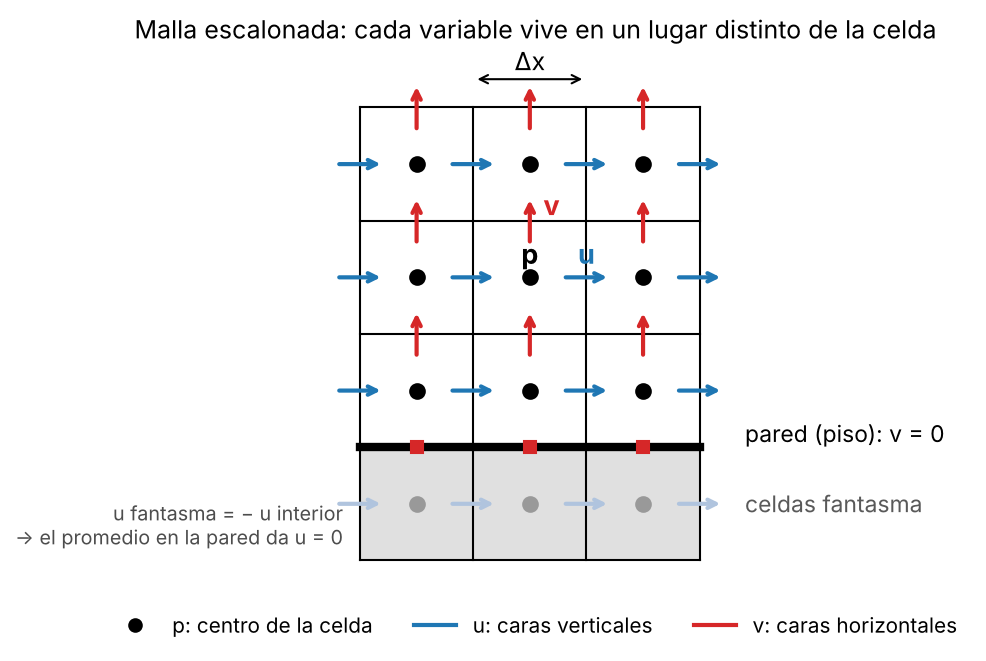
\includegraphics[width=0.55\textwidth]{malla_escalonada.png}
\caption{Malla escalonada: $p$ en el centro, $u$ y $v$ en las caras; fila de celdas fantasma bajo la pared.}
\end{figure}

\subsection{Método de proyección (paso fraccionado de Chorin)}

Sea $\mathbf A(\vu)=\tfrac{1}{\Rey}\nabla^2\vu-\nabla\cdot(\vu\vu)$ el lado derecho de \eqref{eq:ns} sin la presión.
Cada paso de tiempo hace \cite{chorin}:
\begin{align}
&\text{1. Predictor (Adams–Bashforth 2):} && \vu^*=\vu^n+\Delta t\left[\tfrac32\mathbf A(\vu^n)-\tfrac12\mathbf A(\vu^{n-1})\right], \label{eq:pred}\\
&\text{2. Poisson:} && \nabla^2p^{n+1}=\frac{1}{\Delta t}\,\nabla\cdot\vu^*, \label{eq:poisson}\\
&\text{3. Corrector:} && \vu^{n+1}=\vu^*-\Delta t\,\nabla p^{n+1}. \label{eq:corr}
\end{align}
La ecuación \eqref{eq:poisson} se obtiene al aplicar la divergencia a \eqref{eq:corr} y exigir $\nabla\cdot\vu^{n+1}=0$:
\begin{equation}
\nabla\cdot\vu^{n+1}=\nabla\cdot\vu^*-\Delta t\,\nabla^2p^{n+1}=0 .
\end{equation}
Sumando \eqref{eq:pred} y \eqref{eq:corr} se recupera la ecuación de cantidad de movimiento discretizada en el tiempo:
la presión no tiene ecuación propia, es el campo que impone la continuidad.

El predictor estima $\mathbf A$ a la mitad del paso extrapolando linealmente con el paso anterior,
$\mathbf A^{n+1/2}\approx\mathbf A^n+\tfrac12(\mathbf A^n-\mathbf A^{n-1})$ \cite{kimmoin}; en el primer paso, sin
$\mathbf A^{n-1}$, se usa Euler. Con Euler explícito en todos los pasos ($\vu^*=\vu^n+\Delta t\,\mathbf A^n$) y
convección centrada el esquema es inestable: en la prueba de la sección~\ref{sec:dt} explota en 706 pasos.

La matriz de Poisson (5 puntos, Neumann en entrada y paredes, Dirichlet en la salida) no cambia en el tiempo, así que se
factoriza una sola vez (LU dispersa de SciPy) y en cada paso sólo se hace una sustitución. El corrector deja la
divergencia discreta en cero a precisión de máquina.

\subsection{Discretización espacial}

Con $P$ el nodo y $E,W,N,S$ sus vecinos este, oeste, norte y sur:

\paragraph{Difusión.} Laplaciano de 5 puntos, error de truncamiento $O(\Delta x^2)$:
\begin{equation}
\nabla^2u\big|_P\approx\frac{u_E+u_W+u_N+u_S-4u_P}{\Delta x^2}.
\end{equation}

\paragraph{Convección.} En forma conservativa, como ``lo que sale menos lo que entra'' por las caras del volumen de
control de cada velocidad; el valor en cada cara es el promedio de los dos nodos vecinos:
\begin{equation}
\left.\frac{\partial(u^2)}{\partial x}+\frac{\partial(vu)}{\partial y}\right|_P\approx
\frac{\bar u_e^{\,2}-\bar u_w^{\,2}}{\Delta x}+\frac{\bar v_n\bar u_n-\bar v_s\bar u_s}{\Delta x},\qquad
\bar u_e=\tfrac12(u_P+u_E),\quad \bar u_n=\tfrac12(u_P+u_N),
\end{equation}
donde $\bar v_n,\bar v_s$ son promedios de las dos $v$ vecinas de cada cara. Es un esquema centrado, con error
$O(\Delta x^2)$ y sin difusión numérica. Un esquema \emph{upwind} sería más estable, pero añadiría una viscosidad
artificial que acorta la burbuja; con Adams–Bashforth no hace falta.

\paragraph{Divergencia y gradiente.} En la celda $(i,j)$ y en las caras,
\begin{equation}
(\nabla\cdot\vu)_{i,j}=\frac{u_{i+1/2,j}-u_{i-1/2,j}+v_{i,j+1/2}-v_{i,j-1/2}}{\Delta x},\qquad
\left.\frac{\partial p}{\partial x}\right|_{i+1/2,j}=\frac{p_{i+1,j}-p_{i,j}}{\Delta x}.
\end{equation}

\paragraph{Ecuación de Poisson discreta.} Para cada celda con fluido,
\begin{equation}
\sum_{\text{vecinos con fluido}}\frac{p_{\text{vec}}-p_P}{\Delta x^2}=\frac{1}{\Delta t}\,(\nabla\cdot\vu^*)_P .
\end{equation}
Un vecino que es pared, entrada o escalón no se suma ($\partial p/\partial n=0$). En la última columna la cara de salida
está a $\Delta x/2$ del centro y vale $p=0$, de modo que el término es $(0-p_P)/(\Delta x/2)\cdot(1/\Delta x)$: el
coeficiente de $p_P$ aumenta en $-2$. El resultado es un sistema $A\,\mathbf p=\mathbf b$ con una ecuación por celda y
a lo más cinco entradas no nulas por fila.

\subsection{Estabilidad y convergencia}

El paso de tiempo está limitado por la condición CFL convectiva y por la difusiva:
\begin{equation}
\Delta t\le\min\left(\frac{\Delta x}{|u|_{\max}},\;\frac{\Rey}{2}\left(\frac{1}{\Delta x^2}+\frac{1}{\Delta y^2}\right)^{-1}\right).
\end{equation}
Para $\Delta x=0.05$, $|u|_{\max}=1.5$ y $\Rey=200$: $\Delta t_{\text{CFL}}=0.033$ y $\Delta t_{\text{Fo}}=0.125$, así que
manda la convectiva. Por defecto se usa el \SI{50}{\percent} del límite, $\Delta t=0.5\,\Delta x/1.5$. Se declara estado
estacionario cuando
\begin{equation}
\frac{\max|\vu^{n+1}-\vu^n|}{\Delta t}<10^{-4};
\end{equation}
con $10^{-5}$ el valor de $x_r$ cambia menos de \SI{0.3}{\percent}.

\subsection{Post-proceso}

$x_r$ se obtiene como el cruce de $-$ a $+$ de $\tau_w\propto u$ en la primera celda junto a la pared inferior, aguas
abajo del mínimo de $u$ (así no se confunde con el pequeño vórtice de esquina), con interpolación lineal entre nodos. La
burbuja secundaria se detecta igual en la pared superior. La vorticidad $\omega=\partial v/\partial x-\partial u/\partial y$
se calcula en las esquinas de las celdas, donde la malla escalonada la da directamente con diferencias de vecinos.

\paragraph{Tinta virtual.} Para visualizar el transitorio se sueltan partículas sin masa que se mueven con el fluido,
$\dd\mathbf x/\dd t=\vu(\mathbf x,t)$, integradas con Runge–Kutta de segundo orden e interpolación bilineal de la
velocidad. Hay 9 inyectores en la entrada (cada uno de un color, con el tono alternando cada $1\,H/U$ para marcar el
tiempo) y el fluido inicial se marca como un tablero de ajedrez gris.

\subsection{Estructura del código en Python}\label{sec:codigo}

El código está en un solo notebook, \texttt{escalon\_descendente.ipynb}, escrito desde cero con \texttt{numpy} (arreglos
y operaciones vectorizadas), \texttt{scipy.sparse} (matriz de Poisson y factorización LU) y \texttt{matplotlib}
(gráficas y videos). Se ejecuta completo con \emph{Ejecutar todo} y está organizado en bloques:

\begin{enumerate}[label=\textbf{\arabic*.}, start=0]
  \item \textbf{Librerías y parámetros}: \texttt{RE}, \texttt{NY}, \texttt{L} y las constantes de la geometría
    (tabla~\ref{tab:parametros}).
  \item \textbf{La física}: ecuaciones, condiciones de frontera y supuestos (texto).
  \item \textbf{El método numérico} en tres pasos (texto).
  \item \textbf{El código}, función por función (tabla~\ref{tab:funciones}).
  \item \textbf{Caso base} y videos del arranque.
  \item \textbf{Análisis paramétrico}: viscosidad, malla y paso de tiempo.
  \item \textbf{Validación} contra la literatura y conclusiones.
\end{enumerate}

\begin{table}[H]
\centering\small
\caption{Funciones del notebook y la parte del método que implementa cada una.}
\label{tab:funciones}
\begin{tabular}{@{}ll@{}}
\toprule
Función & Qué implementa\\
\midrule
\texttt{crear\_malla} & Malla MAC de $-L_I$ a $L$; marca las celdas sólidas del escalón\\
\texttt{perfil\_entrada} & Perfil de Poiseuille $u=6U\eta(1-\eta)$\\
\texttt{matriz\_presion} & Matriz de Poisson (Neumann/Dirichlet) y su factorización LU\\
\texttt{fronteras} & Condiciones de frontera con celdas fantasma\\
\texttt{aceleracion\_u}, \texttt{aceleracion\_v} & $\mathbf A$: difusión de 5 puntos y convección centrada conservativa\\
\texttt{simular} & Ciclo de tres pasos \eqref{eq:pred}--\eqref{eq:corr}, CFL y criterio de convergencia\\
\texttt{reacoplamiento}, \texttt{burbuja\_superior} & $x_r$ y la burbuja del techo por cambio de signo de $u$\\
\texttt{vorticidad}, \texttt{divergencia\_maxima} & $\omega$ en las esquinas; verificación de $\nabla\cdot\vu\approx0$\\
\texttt{graficar\_campos}, \texttt{animar} & Figuras y videos (tinta virtual)\\
\bottomrule
\end{tabular}
\end{table}

La función central es \texttt{simular(Re, NY, L, dt)}: arma la malla y la matriz, impone la condición inicial y repite
los pasos \eqref{eq:pred}--\eqref{eq:corr} hasta cumplir el criterio de estado estacionario o detectar que la solución
diverge. Cada análisis paramétrico es una llamada a esta función con otros argumentos. El código completo de las
funciones principales está en el anexo~\ref{sec:anexo-codigo}.

% ================================================================
\section{Resultados: caso base \texorpdfstring{$\Rey=200$}{Re = 200}}

\subsection{Ejecución del código}
El caso base se corre con \texttt{base = simular(RE, NY=NY, L=L)}. La salida del notebook es:
\begin{lstlisting}[language={}, numbers=none]
Re =  200 | NY =  20 | dt = 0.0167 | converge  en t =   43.5 (2608 pasos) | x_r/S = 4.91
Divergencia máxima = 5.8e-15   (~ 0: la masa se conserva)
Reacoplamiento: x_r = 2.46 H = 4.91 alturas de escalón
\end{lstlisting}

\subsection{Campos estacionarios}
Con 20 celdas por $H$ (6400 celdas con fluido) y $\Delta t=0.0167$, el estado estacionario se alcanza en
$t=43.5\,H/U$ (2608 pasos, $\sim$\SI{3}{s} de CPU). El reacoplamiento ocurre en $x_r=2.46H$ ($x_r/S=4.91$) y la
divergencia máxima final es \num{5.8e-15}.

\begin{figure}[H]
\centering
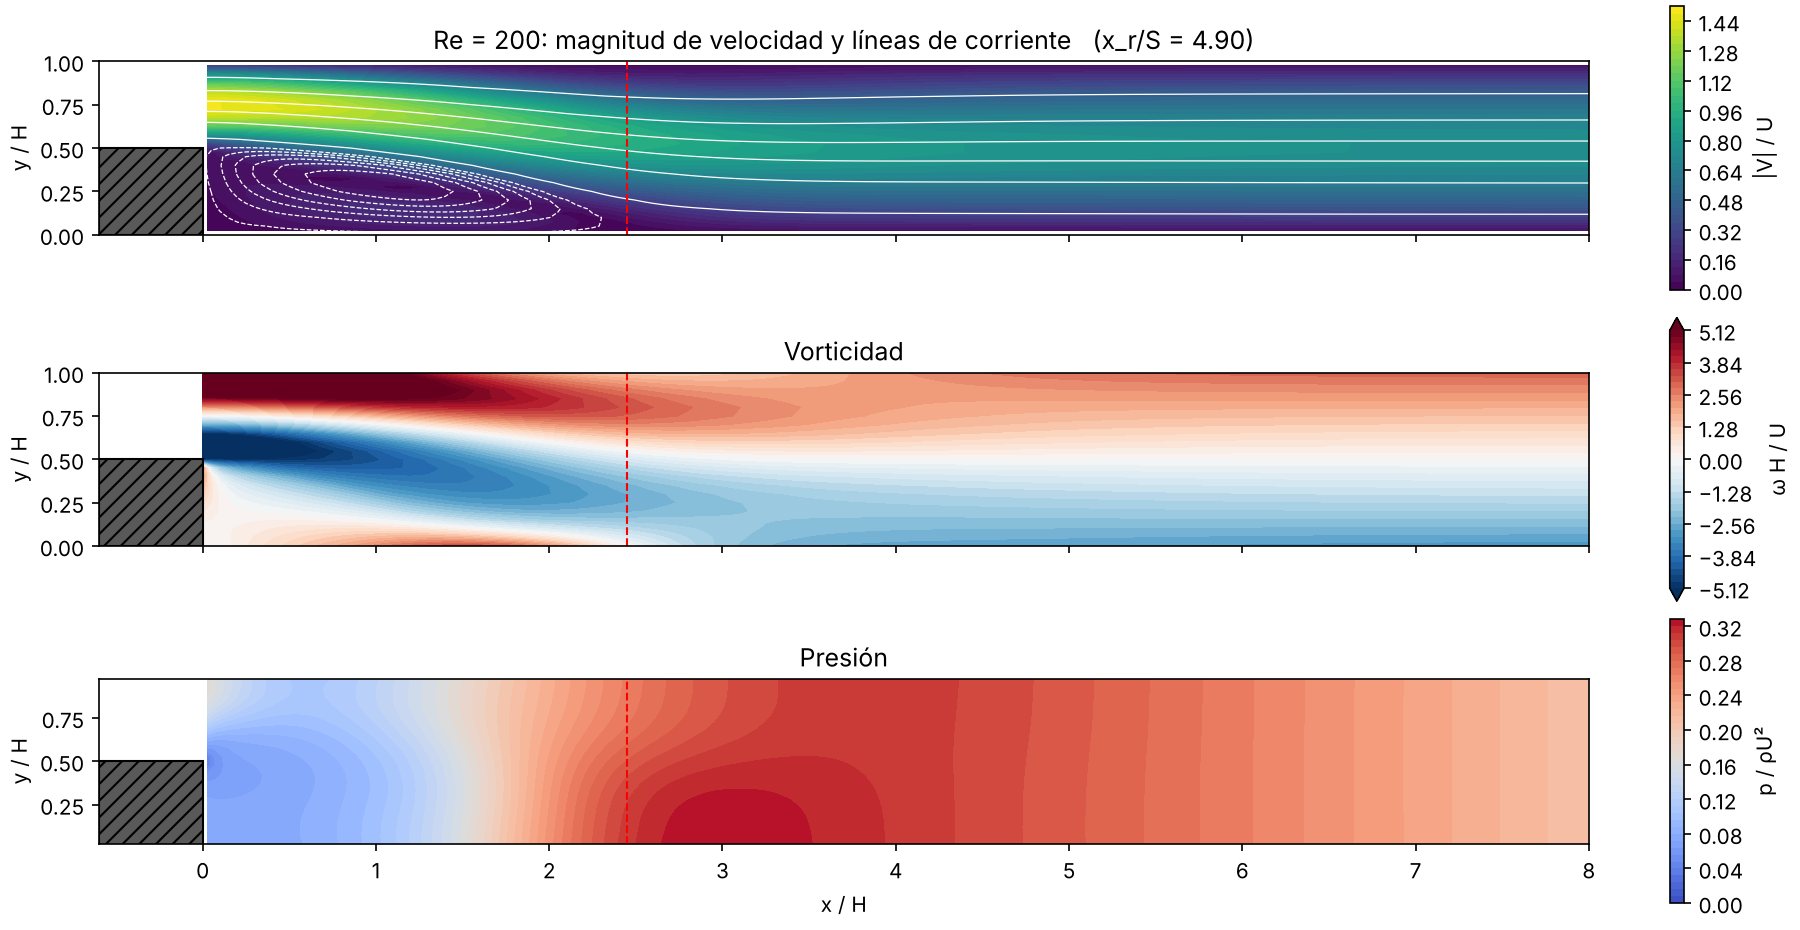
\includegraphics[width=\textwidth]{campos_base.png}
\caption{Campos estacionarios a $\Rey=200$: magnitud de velocidad con líneas de corriente (arriba), vorticidad (centro)
y presión (abajo). La línea roja marca $x_r$.}
\end{figure}

La vorticidad se concentra en la capa de corte que nace en la arista ($\omega<0$) y en la pared superior ($\omega>0$).
La presión es mínima cerca del escalón y \textbf{aumenta} aguas abajo hasta $x\approx3H$: es la recuperación de presión
de la expansión súbita, un gradiente adverso que es justamente la causa de la separación. Después cae linealmente como en
un flujo de Poiseuille desarrollado.

\begin{figure}[H]
\centering
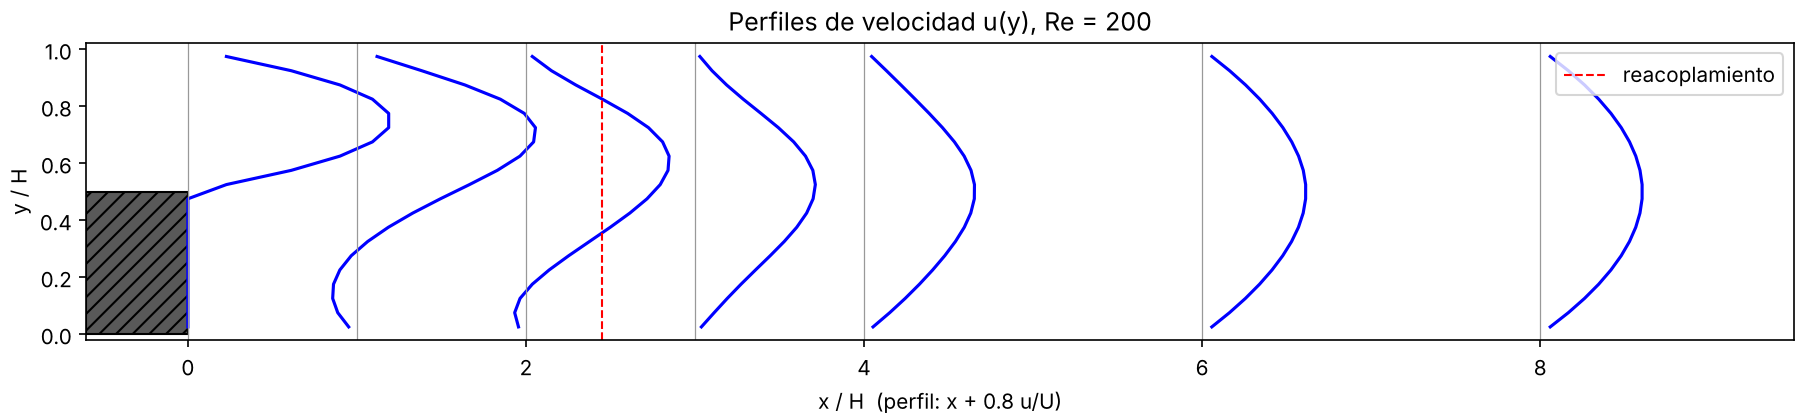
\includegraphics[width=\textwidth]{perfiles_base.png}
\caption{Perfiles $u(y)$ en varias estaciones. El flujo inverso ($u<0$) es visible en $x=1H$ y $2H$.}
\end{figure}

Por conservación de masa la velocidad máxima baja de $1.5U$ (canal de entrada) a $0.75U$ (canal completo).

\subsection{El arranque desde el reposo}

\begin{figure}[H]
\centering
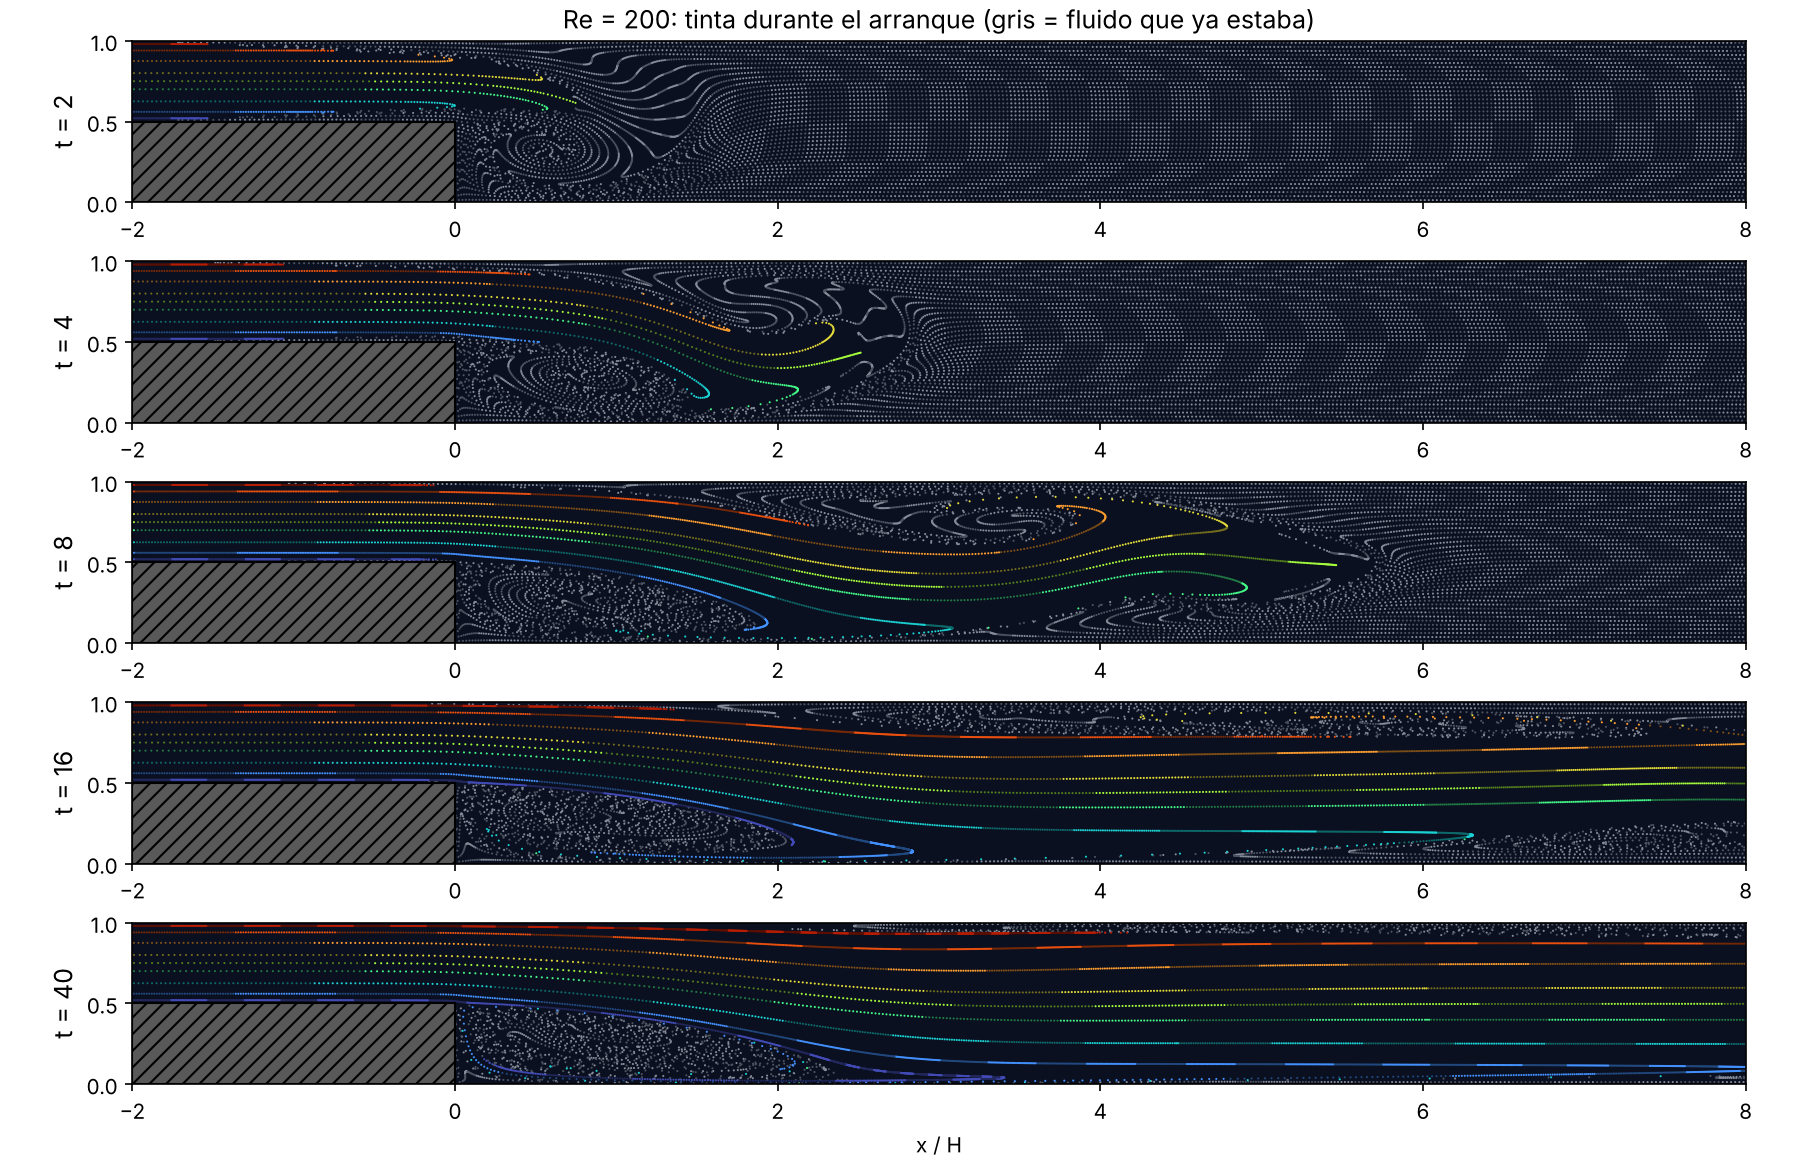
\includegraphics[width=\textwidth]{secuencia_base.png}
\caption{Tinta virtual a $\Rey=200$ (malla de 40 celdas/$H$) en $t=2,4,8,16$ y $40\,H/U$. Gris: fluido que estaba en el
canal al inicio; color: tinta que entra por cada inyector.}
\end{figure}

El video \texttt{figures/arranque\_re200.mp4} (y la secuencia anterior) muestra cómo se forma la burbuja:
\begin{enumerate}
  \item \textbf{Vórtice de arranque} ($t\lesssim5$): la capa de corte que sale de la esquina se enrolla en un vórtice que
    viaja aguas abajo; la tinta toma forma de ``cabeza de hongo''.
  \item \textbf{Separación transitoria en el techo} ($t\approx4$–10): el chorro ondula y despega por un momento el flujo de
    la pared superior, aunque a $\Rey=200$ esa burbuja desaparece en el estado final.
  \item \textbf{Crecimiento lento} del remolino principal: $x_r$ llega al \SI{90}{\percent} de su valor final en
    $t\approx11\,H/U$ y se estabiliza en $t\approx40$.
  \item \textbf{Fluido atrapado:} el fluido gris que quedó dentro de la burbuja gira en su lugar y nunca sale; la tinta
    pasa por encima. Es la definición de zona de recirculación.
\end{enumerate}
En \texttt{figures/comparacion\_re.mp4} se ven los arranques de $\Rey=100$, 300 y 600 en paralelo. A $\Rey=100$ el flujo
se calma en $t\approx20$; a $\Rey=600$ se forman varios vórtices que viajan y se fusionan, y la burbuja del techo aparece
y se queda.

% ================================================================
\section{Análisis paramétrico}

\subsection{Viscosidad (número de Reynolds)}

Se varía $\nu=1/\Rey$ con 20 celdas/$H$ y $L=25H$, para que el remolino no llegue a la salida.

\begin{table}[H]
\centering\small
\caption{Longitud de reacoplamiento y burbuja superior contra $\Rey$.}
\label{tab:re}
\begin{tabular}{@{}rrrrl@{}}
\toprule
$\Rey$ & $\nu$ & $x_r/S$ & Pasos & Burbuja superior, $x/H$\\
\midrule
100 & 0.0100 & 2.84 & 1194 & ---\\
200 & 0.0050 & 4.91 & 2608 & ---\\
300 & 0.0033 & 6.73 & 4889 & ---\\
400 & 0.0025 & 8.26 & 8294 & 4.20 -- 4.50 (incipiente)\\
500 & 0.0020 & 9.40 & 12997 & 4.00 -- 6.30\\
600 & 0.0017 & 10.06 & 17338 & 4.05 -- 7.60\\
\bottomrule
\end{tabular}
\end{table}

\begin{figure}[H]
\centering
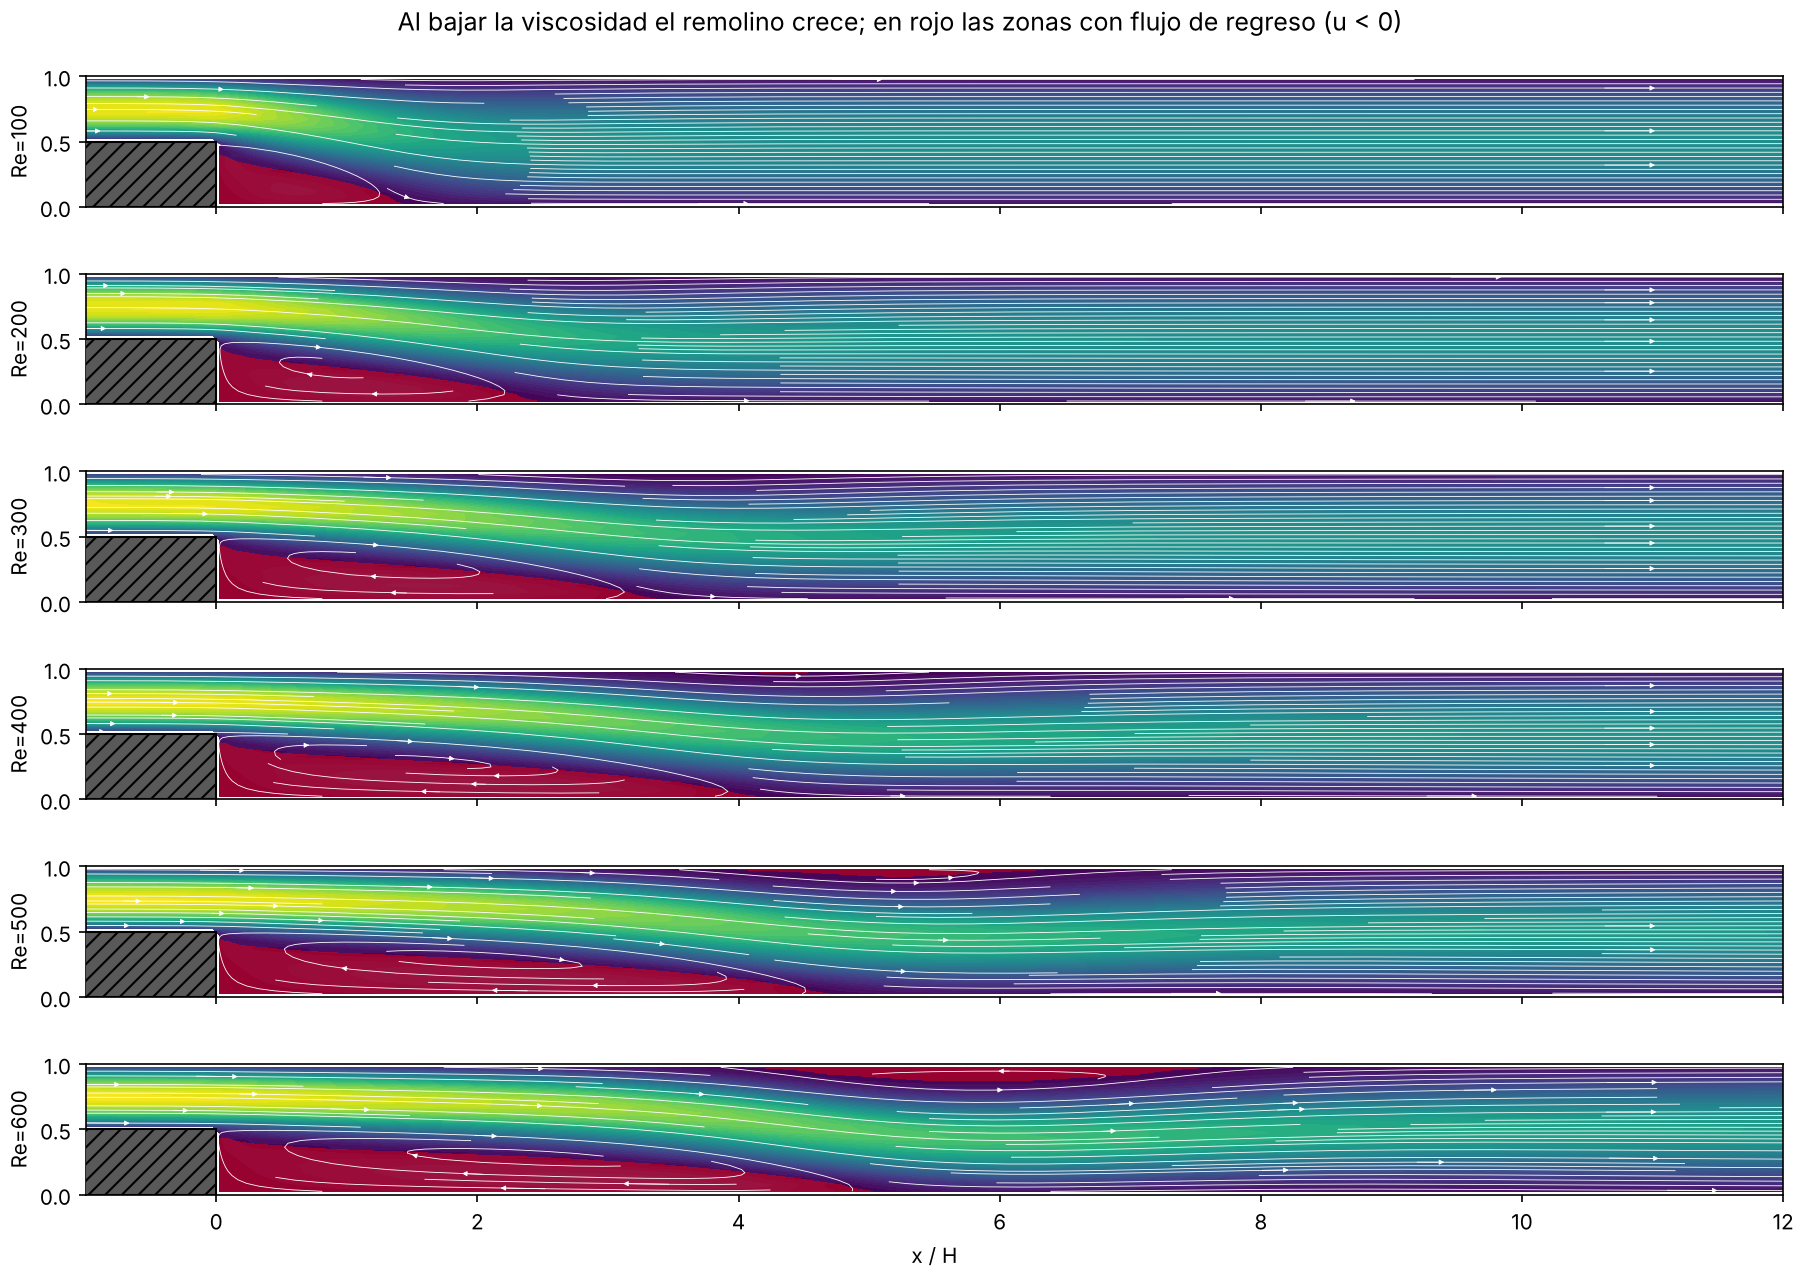
\includegraphics[width=0.92\textwidth]{re_remolinos.png}
\caption{Velocidad y líneas de corriente para $\Rey=100$ a 600. En rojo, zonas de flujo inverso ($u<0$).}
\end{figure}

\begin{figure}[H]
\centering
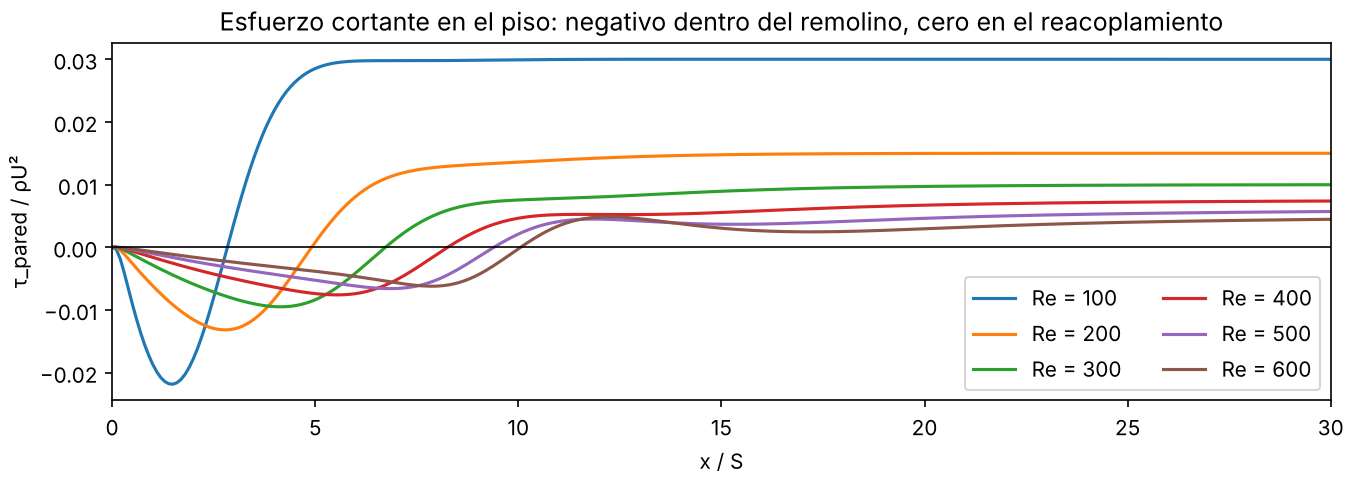
\includegraphics[width=0.75\textwidth]{re_cortante.png}
\caption{Esfuerzo cortante en la pared inferior. Cada curva cruza cero en su $x_r$.}
\end{figure}

Al bajar la viscosidad la burbuja principal se alarga casi linealmente con $\Rey$ hasta $\sim$400 y después crece más
lento, cuando aparece la burbuja superior: ésta estrecha el paso del flujo principal, lo empuja hacia abajo y limita el
crecimiento de la burbuja inferior. El mínimo de $\tau_w$ dentro de la burbuja se hace menos negativo con $\Rey$ porque
$\tau_w\propto\nu$. El tiempo para llegar al estado estacionario también crece con $\Rey$ (de $t=19.9$ a $t=289$): el
transitorio lo controla la difusión viscosa.

\subsection{Velocidad de entrada}

En forma adimensional la velocidad de entrada no es un parámetro independiente: $U$ sólo aparece en $\Rey=UH/\nu$.
\textbf{Aumentar la velocidad de entrada con la misma viscosidad es lo mismo que aumentar $\Rey$} (similitud dinámica):
duplicar $U$ duplica $\Rey$ y produce el mismo flujo adimensional que reducir $\nu$ a la mitad; lo único que cambia es la
escala de tiempo $H/U$. Por eso el barrido de la tabla~\ref{tab:re} es también un barrido en velocidad. Como ejemplo,
para agua ($\nu\approx\SI{1e-6}{m^2/s}$) en un canal de $H=\SI{1}{cm}$, $\Rey=100$ a 600 corresponde a
$U=\Rey\,\nu/H=\SI{1}{cm/s}$ a \SI{6}{cm/s}: el remolino pasa de $x_r/S=2.84$ a $10.06$.

En la estabilidad, mayor velocidad (mayor $\Rey$) no reduce el $\Delta t$ adimensional permitido por el CFL, porque la
velocidad máxima sigue siendo $1.5U$; sí aumenta el límite difusivo ($\Delta t_{\text{Fo}}\propto\Rey$) y, sobre todo,
alarga el transitorio: de 1194 pasos a $\Rey=100$ a \num{17338} a $\Rey=600$.

\subsection{Malla}

\begin{table}[H]
\centering\small
\caption{Estudio de malla a $\Rey=200$.}
\label{tab:malla}
\begin{tabular}{@{}rrrr@{}}
\toprule
Celdas por $H$ & Celdas con fluido & $x_r/S$ & CPU\\
\midrule
10 & 1600 & 4.754 & $\sim$\SI{0.5}{s}\\
20 & 6400 & 4.914 & $\sim$\SI{3}{s}\\
40 & 25600 & 4.946 & $\sim$\SI{30}{s}\\
\bottomrule
\end{tabular}
\end{table}

Al duplicar la malla el cambio en $x_r$ se reduce unas 5 veces ($+0.160$ y luego $+0.032$). Con razón de refinamiento 2,
el orden observado y la extrapolación de Richardson son
\begin{equation}
p=\log_2\frac{x_{20}-x_{10}}{x_{40}-x_{20}}\approx2.3,\qquad
x_\infty\approx x_{40}+\frac{x_{40}-x_{20}}{2^p-1}\approx4.95\,S,
\end{equation}
consistente con el orden formal 2 del esquema. El error con 20 celdas/$H$ es $\approx$\SI{0.8}{\percent}. El costo crece
$\sim$10$\times$ por cada refinamiento (4$\times$ celdas y 2$\times$ pasos por el CFL).

\begin{figure}[H]
\centering
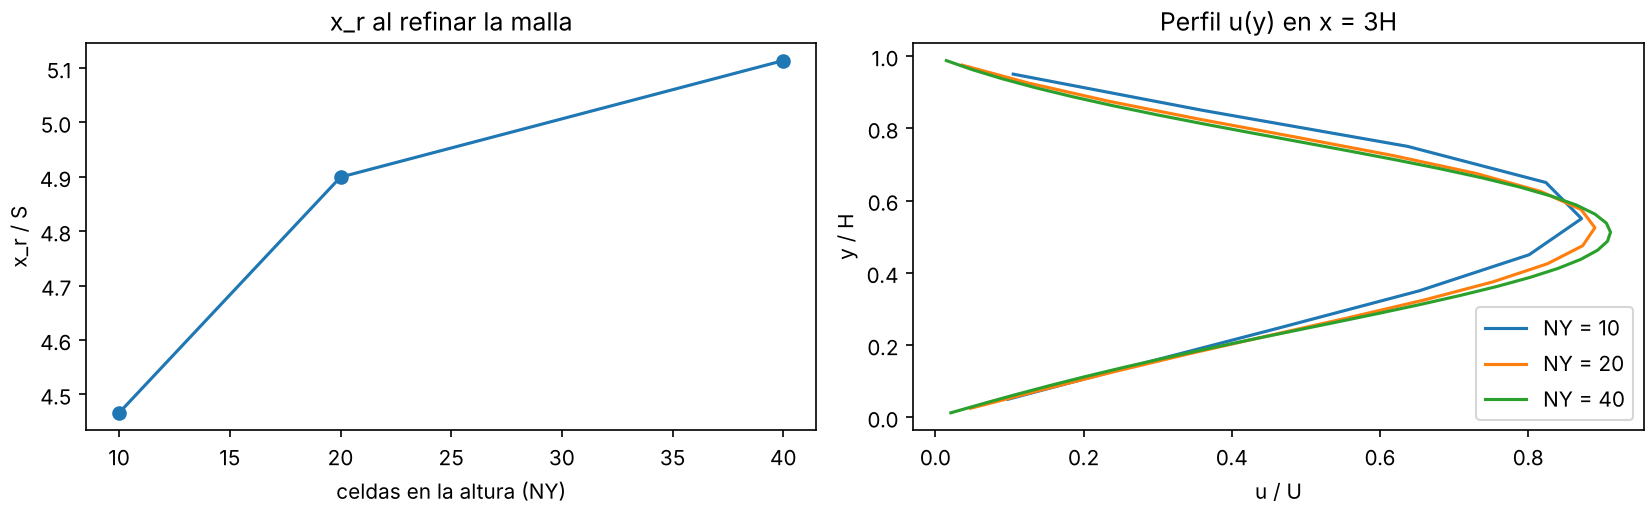
\includegraphics[width=0.85\textwidth]{malla.png}
\caption{Cambio de $x_r$ con la malla y perfil $u(y)$ en $x=1H$, dentro del remolino.}
\end{figure}

\subsection{Paso de tiempo y estabilidad}\label{sec:dt}

Para $\Rey=200$ y 20 celdas/$H$: $\Delta t_{\text{CFL}}=0.033$ y $\Delta t_{\text{Fo}}=0.125$, de modo que manda el CFL.

\begin{table}[H]
\centering\small
\caption{Efecto del paso de tiempo.}
\label{tab:dt}
\begin{tabular}{@{}rrlrr@{}}
\toprule
$\Delta t$ & $\Delta t/\Delta t_{\text{CFL}}$ & Resultado & Pasos & $x_r/S$\\
\midrule
0.0083 & 0.25 & converge & 5215 & 4.914\\
0.0167 & 0.50 & converge & 2608 & 4.914\\
0.0267 & 0.80 & converge & 1631 & 4.914\\
0.0333 & 1.00 & \textbf{diverge} en 36 pasos & --- & ---\\
0.0167 (Euler) & 0.50 & \textbf{diverge} en 706 pasos & --- & ---\\
\bottomrule
\end{tabular}
\end{table}

\begin{figure}[H]
\centering
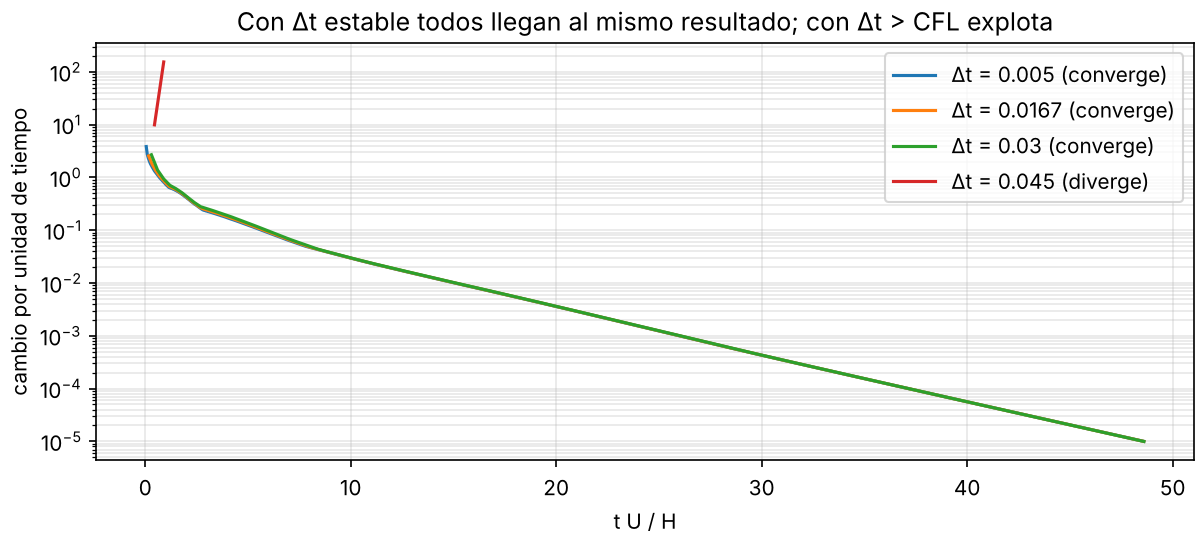
\includegraphics[width=0.72\textwidth]{dt.png}
\caption{Historia del residuo $\max|\vu^{n+1}-\vu^n|/\Delta t$ para distintos $\Delta t$.}
\end{figure}

El estado estacionario es \textbf{independiente de $\Delta t$} mientras el esquema sea estable; un $\Delta t$ mayor sólo
reduce el número de pasos. En el límite CFL el error crece exponencialmente y la solución explota. Euler explícito
explota incluso con la mitad del límite: con convección centrada necesita Adams–Bashforth.

% ================================================================
\section{Validación}

\begin{figure}[H]
\centering
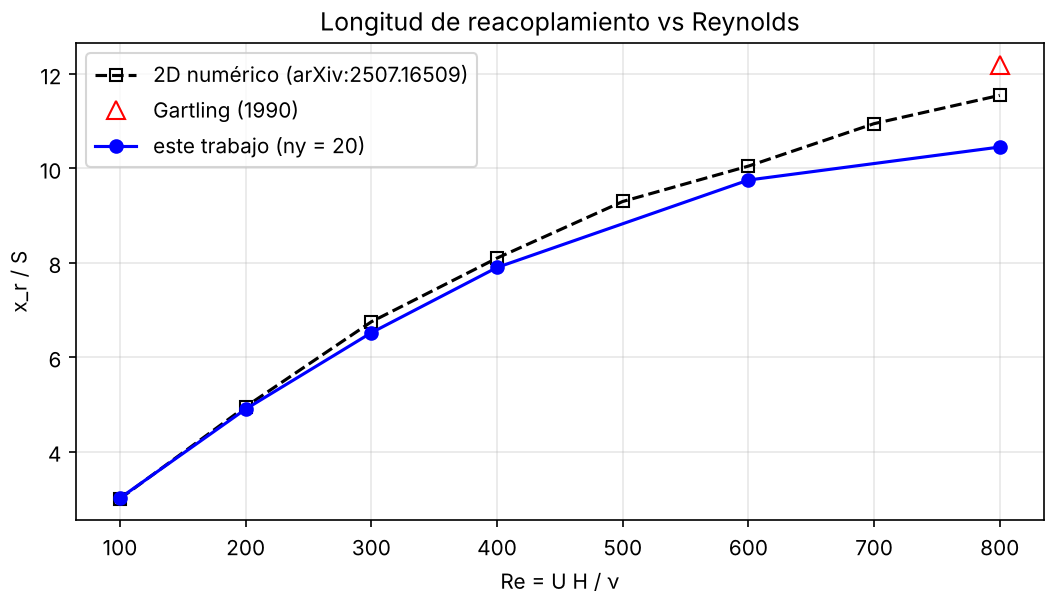
\includegraphics[width=0.68\textwidth]{validacion.png}
\caption{Longitud de reacoplamiento contra Reynolds: este trabajo y la literatura.}
\end{figure}

\begin{table}[H]
\centering\small
\caption{Comparación con simulaciones 2D publicadas \cite{arxiv}.}
\label{tab:val}
\begin{tabular}{@{}rrrr@{}}
\toprule
$\Rey$ & Este trabajo & Referencia 2D & Diferencia\\
\midrule
100 & 2.84 & 3.00 & $-5.4$\,\%\\
200 & 4.91 & 4.95 & $-0.7$\,\%\\
300 & 6.73 & 6.75 & $-0.3$\,\%\\
400 & 8.26 & 8.10 & $+2.0$\,\%\\
500 & 9.40 & 9.30 & $+1.1$\,\%\\
600 & 10.06 & 10.05 & $+0.1$\,\%\\
\bottomrule
\end{tabular}
\end{table}

Para $200\le\Rey\le600$ las diferencias son de \SI{2}{\percent} o menos, y se reproduce el remolino del techo a partir de
$\Rey\approx400$. Como el error de malla es menor a \SI{1}{\percent}, estas diferencias son del orden de la dispersión
entre los propios estudios publicados (que difieren en el largo del canal de entrada y del dominio). La mayor diferencia,
en $\Rey=100$, ocurre donde la burbuja es más corta y más sensible al perfil que llega a la esquina.

% ================================================================
\section{Conclusiones}

\subsection{Interpretación física}
\begin{enumerate}
  \item La separación en la esquina se explica por el \textbf{gradiente de presión adverso}: al ensancharse el canal el
    fluido se frena y la presión sube hasta $x\approx3H$; el fluido lento junto a la pared no puede avanzar contra ese
    aumento y se despega.
  \item La longitud del remolino la fija la competencia entre \textbf{convección y difusión viscosa}: con menos viscosidad
    (mayor $\Rey$) el chorro transmite su momento hacia el piso más lentamente mientras la convección lo lleva más lejos,
    así que $x_r/S$ crece de 2.84 a 10.06 entre $\Rey=100$ y 600, casi linealmente hasta $\Rey\approx400$.
  \item Desde $\Rey\approx400$ también se separa la capa límite del techo; esa \textbf{burbuja secundaria} estrecha el paso
    del chorro, lo empuja hacia abajo y frena el crecimiento de la burbuja principal.
  \item La recirculación es una región cerrada: el fluido que queda atrapado en ella gira sin salir (tinta virtual), y el
    reacoplamiento coincide con $\tau_w=0$.
  \item Por continuidad la velocidad máxima baja de $1.5U$ a $0.75U$ aguas abajo, donde el perfil vuelve a ser parabólico.
\end{enumerate}

\subsection{Alcances}
\begin{itemize}
  \item El código resuelve Navier–Stokes 2D incompresible con el método de proyección, conserva la masa a precisión de
    máquina ($\sim10^{-15}$) y es de segundo orden en el espacio (orden observado 2.3; error de malla $<\SI{1}{\percent}$
    con 20 celdas/$H$).
  \item Reproduce el transitorio desde el reposo y el estado estacionario para cualquier $\Rey$ entre 100 y 600 cambiando un
    solo parámetro, con diferencias de \SI{2}{\percent} o menos frente a la literatura para $200\le\Rey\le600$.
  \item El análisis de estabilidad es cuantitativo: dentro del límite CFL el resultado no depende de $\Delta t$; en el límite
    o con Euler explícito el método diverge.
  \item Como el escalón es una máscara de celdas sólidas, la misma estructura sirve para otras geometrías rectangulares
    (otra altura de escalón u obstáculos) cambiando \texttt{crear\_malla} y \texttt{fronteras}.
\end{itemize}

\subsection{Limitaciones}
\begin{itemize}
  \item \textbf{Bidimensional.} El flujo real se vuelve tridimensional para $\Rey\gtrsim400$ \cite{armaly}; por eso
    comparamos con simulaciones 2D y no directamente con los experimentos a $\Rey$ alto.
  \item \textbf{Laminar y estacionario.} No hay modelo de turbulencia; el modelo deja de ser válido cerca de la transición
    ($\Rey\approx1200$).
  \item \textbf{Resolución.} La malla es uniforme y no se refina cerca de la esquina. A $\Rey=800$ (fuera del rango
    estudiado) obtuvimos $x_r/S=10.71$ con 20 celdas/$H$ frente a 11.55 de la literatura ($-\SI{7}{\percent}$): a
    $\Rey$ alto hacen falta más celdas.
  \item \textbf{Costo del método explícito.} El CFL limita $\Delta t$: cada vez que se duplica la malla el costo crece
    $\sim$10 veces, y el estado estacionario se alcanza marchando en el tiempo (\num{17338} pasos a $\Rey=600$).
  \item \textbf{Condiciones de frontera idealizadas.} La entrada supone un perfil de Poiseuille ya desarrollado a $2H$ del
    escalón, y la salida exige un canal más largo que el remolino ($L=25H$). Ambas influyen en $x_r$; la mayor
    diferencia con la literatura ($-\SI{5.4}{\percent}$ a $\Rey=100$) ocurre donde la burbuja es más sensible al perfil
    de entrada.
  \item \textbf{Propiedades constantes}: fluido newtoniano, isotérmico y sin gravedad.
\end{itemize}

% ================================================================
\begin{thebibliography}{9}\small
\bibitem{armaly} B.~F.~Armaly, F.~Durst, J.~C.~F.~Pereira, B.~Schönung (1983). Experimental and theoretical
  investigation of backward-facing step flow. \emph{J.\ Fluid Mech.}\ 127, 473--496.
\bibitem{gartling} D.~K.~Gartling (1990). A test problem for outflow boundary conditions---flow over a backward-facing
  step. \emph{Int.\ J.\ Numer.\ Methods Fluids} 11, 953--967.
\bibitem{chorin} A.~J.~Chorin (1968). Numerical solution of the Navier–Stokes equations. \emph{Math.\ Comp.}\ 22,
  745--762.
\bibitem{harlow} F.~H.~Harlow, J.~E.~Welch (1965). Numerical calculation of time-dependent viscous incompressible flow
  of fluid with free surface. \emph{Phys.\ Fluids} 8, 2182--2189.
\bibitem{kimmoin} J.~Kim, P.~Moin (1985). Application of a fractional-step method to incompressible Navier–Stokes
  equations. \emph{J.\ Comput.\ Phys.}\ 59, 308--323.
\bibitem{arxiv} arXiv:2507.16509 (2025). A Finite Volume and Levenberg–Marquardt Optimization Framework for
  Benchmarking MHD Flows over Backward-Facing Steps (Tabla 1).
\bibitem{kangluosee} kangluosee. \emph{CFD-Python: Combined backward facing step} (GitHub). Referencia del problema; el
  código de este proyecto se escribió desde cero.
\end{thebibliography}

% ================================================================
\appendix
\section{Uso del código}

\begin{lstlisting}[language=bash, numbers=none]
pip install numpy scipy matplotlib jupyter imageio-ffmpeg
jupyter notebook escalon_descendente.ipynb      # Kernel -> Restart & Run All
\end{lstlisting}
Los parámetros de la demostración en vivo (\texttt{RE}, \texttt{NY}, \texttt{L}) están en el bloque~0. Con
\texttt{HACER\_VIDEOS = False} el notebook se salta los videos y corre en $\sim$3 min. Las figuras se guardan en
\texttt{figures/}.

La correspondencia entre las funciones y el método está en la tabla~\ref{tab:funciones}.

\section{Código fuente de las funciones principales}\label{sec:anexo-codigo}

\lstset{basicstyle=\ttfamily\scriptsize}
El código de esta sección se extrae automáticamente del notebook final al compilar el reporte
(\texttt{reporte/build\_pdf.py}).

\subsection*{Malla y perfil de entrada}
\lstinputlisting{codigo/crear_malla.py}
\lstinputlisting{codigo/perfil_entrada.py}

\subsection*{Matriz de la ecuación de Poisson}
\lstinputlisting{codigo/matriz_presion.py}

\subsection*{Condiciones de frontera}
\lstinputlisting{codigo/fronteras.py}

\subsection*{Convección y difusión (ecuación de $x$; la de $y$ es análoga)}
\lstinputlisting{codigo/aceleracion_u.py}

\subsection*{El ciclo de tres pasos}
\lstinputlisting{codigo/simular.py}

\subsection*{Post-proceso}
\lstinputlisting{codigo/reacoplamiento.py}
\lstinputlisting{codigo/vorticidad.py}

\end{document}
